\documentclass{article}

\usepackage{graphicx}
\usepackage{amsmath}
\usepackage{amssymb}
\usepackage{caption}
\usepackage[utf8]{inputenc}
\usepackage{listings}
\usepackage{xcolor}

% Define Python listing style
\lstdefinestyle{python}{
    language=Python,
    basicstyle=\scriptsize\ttfamily,
    keywordstyle=\color{blue}\bfseries,
    stringstyle=\color{red},
    commentstyle=\color{gray}\itshape,
    showstringspaces=false,
    frame=single,
    breaklines=true,
    columns=fullflexible
}

\renewcommand{\figurename}{Figura}

\begin{document}

\begin{flushleft}
    \LARGE Banjercito \\[6pt]
    \Large Diplomado en Ciencia de Datos
\end{flushleft}

\vfill

\begin{flushleft}
    \LARGE \textbf{Guía de Estudio} \\[12pt]
    \LARGE Evaluación Final \\[24pt]
\end{flushleft}

\vfil

\begin{flushleft}
    Alan Badillo Salas \\[12pt]
    \scriptsize Diciembre 2024 \\[24pt]
\end{flushleft}

\vfill

\section*{Introducción}

El Diplomado en Ciencia de Datos ha llegado a su etapa final, dentro del diplomado hemos aprendido a lo largo de 5 módulos, el uso de las herramientas más importantes usadas en el campo de la ciencia de datos. En el primer módulo hemos introducido el análisis financiero a través de Excel, Power BI y Python, en el segundo módulo hemos reunido los conceptos más importantes de probabilidad y estadística, en el tercer módulo hemos trabajado más a detalle con las librerías de Numpy y Pandas y el flujo de la ciencia de datos, en el cuarto módulo hemos aprendido las tres piezas fundamentales del Machine Learning, que son la Regresión, la Clasificación y la Clusterización, así como la simulación estadística y probabilística, finalmente, en el quinto módulo hemos generalizado todos los modelos, para que una Red Neuronal pueda hacer los pronósticos generalizados a través del Deep Learning.
\\[12pt]
En esta guía repasaremos los fundamentos de cada módulo, a través de preguntas y reactivos similares a los de la evaluación final del diplomado, cubriendo los conceptos vistos en cada módulo y detallando su solución. Comprender esta guía debería ser suficiente para tener un buen desempeño como Científico de Datos y estar preparado para problemas del mercado actual y aplicaciones reales en la industria y el gobierno.

\clearpage

\section*{Módulo I | Introducción a Python con Finanzas}

\subsection*{Problema 1 | Uso de Excel}

Una empresa financiera posee una tabla con los montos de créditos que ha aprobado a sus clientes. La tabla posee el género de cada cliente y se desea calcular el monto total de los créditos aprobados para hombres y mujeres.
\\[12pt]
En la Figura \ref{fig:p101-1} se muestra la tabla con el cliente, género, crédito y monto aprobado.
\begin{figure}[!ht]
    \centering
    \begin{minipage}{\textwidth}
        \centering
        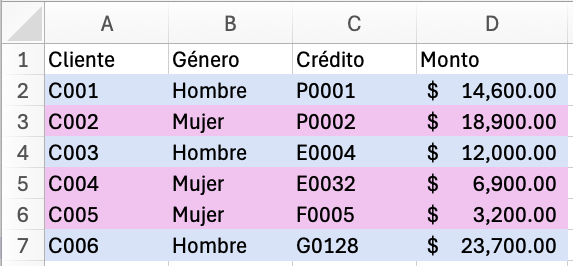
\includegraphics[width=\textwidth]{figures/p101-1.png}
    \end{minipage}
    % \hfill
    % \begin{minipage}{0.4\textwidth}
    %     \centering
    %     \includegraphics[width=\textwidth]{figures/d001.png}
    % \end{minipage}
    % \hfill
    \captionsetup{width=0.9\textwidth}
    \caption{Créditos aprobados a clientes por género}
    \label{fig:p101-1}
\end{figure}
\\
(a) Calcule la suma suma de los montos para hombres y la suma de montos para mujeres usando la fórmula \texttt{=SUMA.SI(RANGO CRITERIO, CRITERIO, RANGO SUMA)}.
\\[6pt]
(b) Calcule la suma suma de los montos para hombres y la suma de montos para mujeres usando la fórmula \texttt{=SUMA(FILTRAR(RANGO SUMA, RANGO INCLUIR))}.

\clearpage

\subsubsection*{Solución al Problema 1}

Para el inciso (a) utilizamos las fórmulas
\\[12pt]
\texttt{=SUMAR.SI(B2:B7,"HOMBRE",D2:D7)}
\\[0pt]
\texttt{=SUMAR.SI(B2:B7,"MUJER",D2:D7)}
\begin{figure}[!ht]
    \centering
    \begin{minipage}{\textwidth}
        \centering
        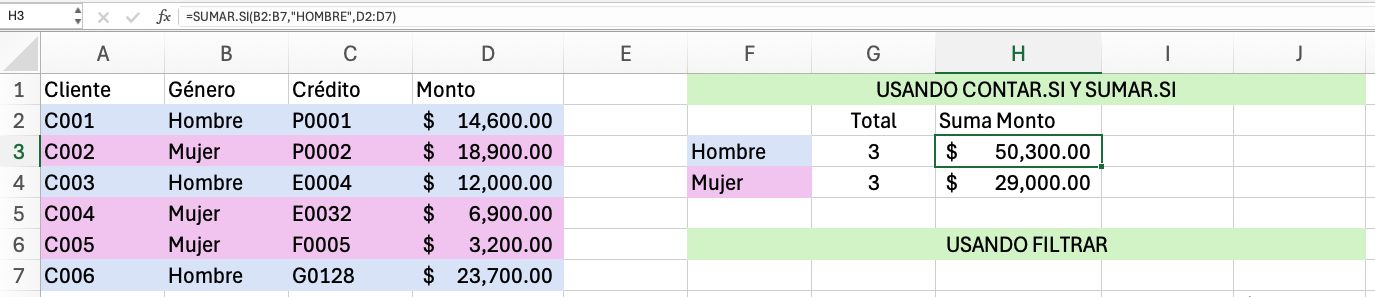
\includegraphics[width=\textwidth]{figures/s101-1a1.png}
    \end{minipage}
    \hfill
    \begin{minipage}{\textwidth}
        \centering
        
\includegraphics[width=\textwidth]{figures/s101-1a2.png}
    \end{minipage}
    \captionsetup{width=0.9\textwidth}
    \caption{Solución al Problema 1 inciso (a)}
    \label{fig:s101-1a}
\end{figure}

\noindent
Para el inciso (b) utilizamos las fórmulas
\\[12pt]
\texttt{=SUMA(FILTRAR(D2:D7,B2:B7="HOMBRE"))}
\\[0pt]
\texttt{=SUMA(FILTRAR(D2:D7,B2:B7="MUJER"))}
\begin{figure}[!ht]
    \centering
    \begin{minipage}{\textwidth}
        \centering
        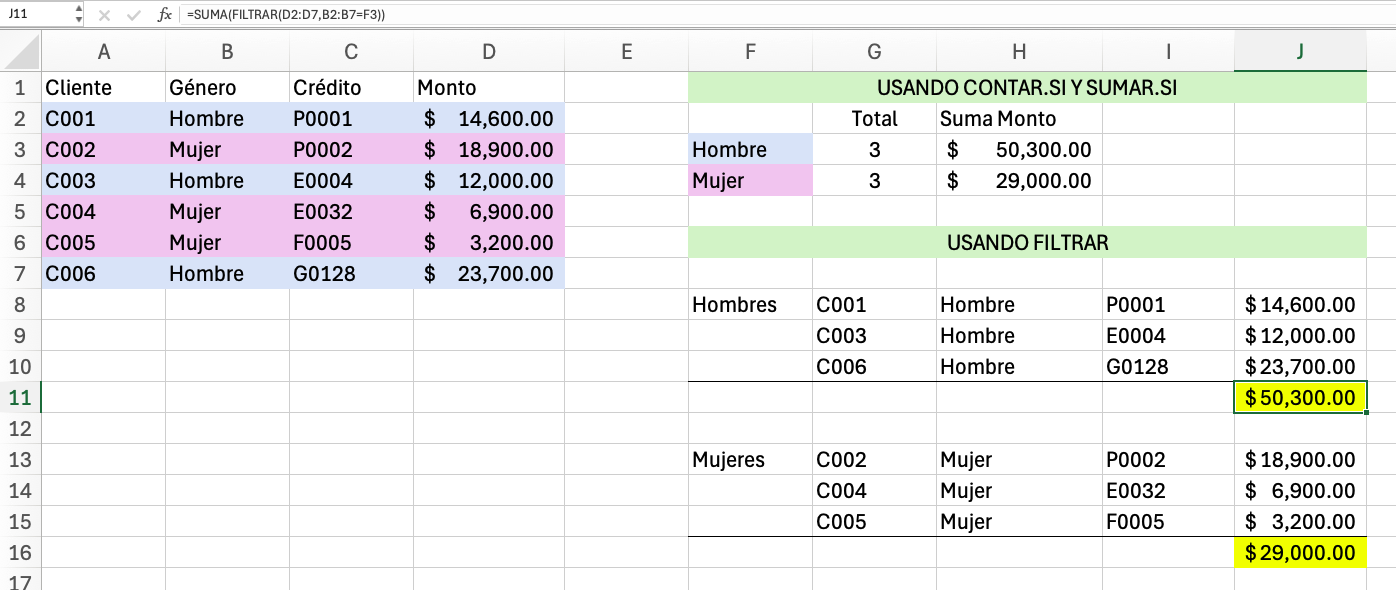
\includegraphics[width=\textwidth]{figures/s101-1b1.png}
    \end{minipage}
    \hfill
    \begin{minipage}{\textwidth}
        \centering
        
\includegraphics[width=\textwidth]{figures/s101-1b2.png}
    \end{minipage}
    \captionsetup{width=0.9\textwidth}
    \caption{Solución al Problema 1 inciso (b)}
    \label{fig:s101-1b}
\end{figure}

\noindent
Nota: Si se utilizamos las fórmulas
\\[12pt]
\texttt{=FILTRAR(A2:D7,B2:B7="HOMBRE")}
\\[0pt]
\texttt{=FILTRAR(A2:D7,B2:B7="HOMBRE")}
\\[12pt]
Se generará la tabla virtual con todos los créditos correspondientes a las filas de los hombres o de las mujeres.
\begin{figure}[!ht]
    \centering
    \begin{minipage}{\textwidth}
        \centering
        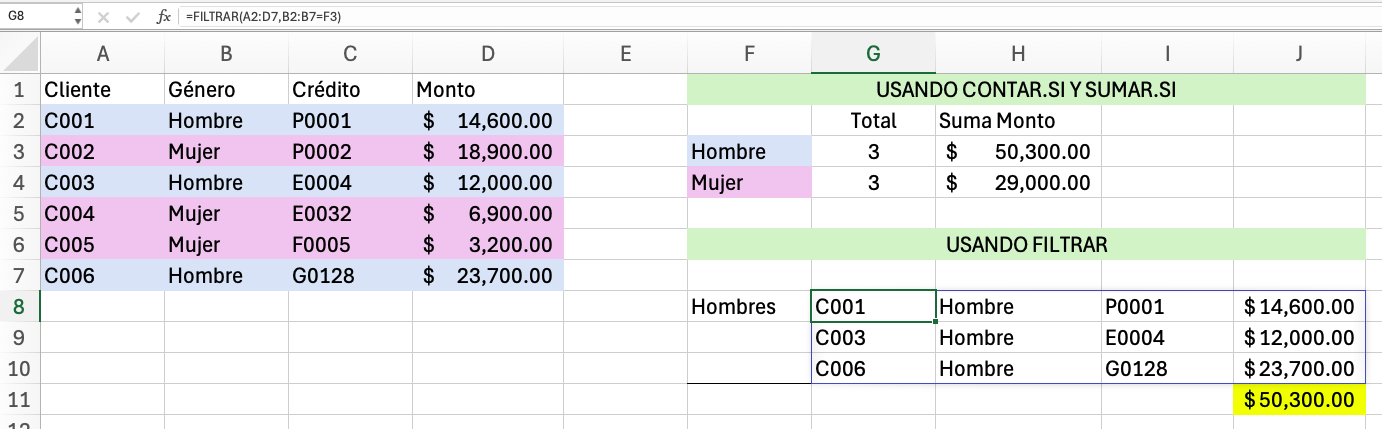
\includegraphics[width=\textwidth]{figures/s101-2.png}
    \end{minipage}
    \hfill
    \begin{minipage}{\textwidth}
        \centering
        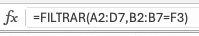
\includegraphics[width=\textwidth]{figures/s101-3.png}
    \end{minipage}
    \hfill
    \begin{minipage}{\textwidth}
        \centering
        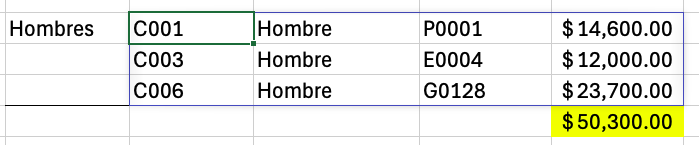
\includegraphics[width=\textwidth]{figures/s101-4.png}
    \end{minipage}
    \captionsetup{width=0.9\textwidth}
    \caption{Tabla virtual generada por FILTRAR (c)}
    \label{fig:s101-c}
\end{figure}

\clearpage

\subsection*{Problema 2 | Uso de Tablas dinámicas en Excel}

Una empresa financiera posee una tabla con los montos de créditos que ha aprobado a sus clientes y su deuda actual. La tabla posee el género de cada cliente y se desea calcular la deuda total y deuda promedio.
\\[12pt]
En la Figura \ref{fig:p102} se muestra la tabla con el cliente, género, crédito, monto aprobado y deuda actual.
\begin{figure}[!ht]
    \centering
    \begin{minipage}{\textwidth}
        \centering
        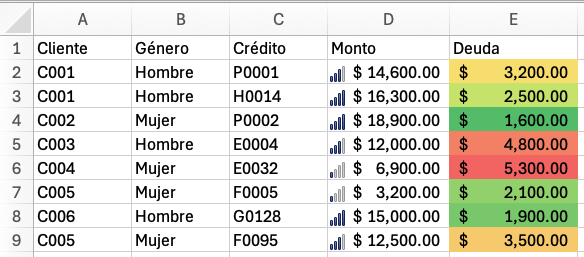
\includegraphics[width=\textwidth]{figures/p102.png}
    \end{minipage}
    % \hfill
    % \begin{minipage}{0.4\textwidth}
    %     \centering
    %     \includegraphics[width=\textwidth]{figures/d001.png}
    % \end{minipage}
    % \hfill
    \captionsetup{width=0.9\textwidth}
    \caption{Créditos aprobados con deuda actual a clientes por género}
    \label{fig:p102}
\end{figure}
\\
(a) Crea una tabla dinámica de \texttt{A1:E9}.
\\[6pt]
(b) Segmenta las filas por Género y luego por Cliente.
\\[6pt]
(c) Cuenta el número de Créditos en valores.
\\[6pt]
(d) Calcula la suma del Monto en valores.
\\[6pt]
(e) Calcula la suma de la Deuda en valores.
\\[6pt]
(f) Calcula el promedio del Monto en valores.
\\[6pt]
(g) Calcula el promedio de la Deuda en valores.
\\[6pt]
(h) ¿Quién es el cliente de mayor deuda?
\\[6pt]
(i) ¿Quién es el cliente al que se le ha prestado más en promedio?
\\[6pt]
(j) ¿Quién es el cliente hombre con mayor deuda promedio?
\\[6pt]
(k) ¿Es significativamente distinta la deuda entre hombres y mujeres?
\\[6pt]
(l) ¿Cuánto se ha recuperado en total de todos los créditos?

\clearpage

\subsubsection*{Solución al Problema 2}

Para el inciso (a) creamos la tabla dinámica para el rango \texttt{A1:E9} y la insertamos en una celda de la misma hoja.
\begin{figure}[!ht]
    \centering
    \begin{minipage}{\textwidth}
        \centering
        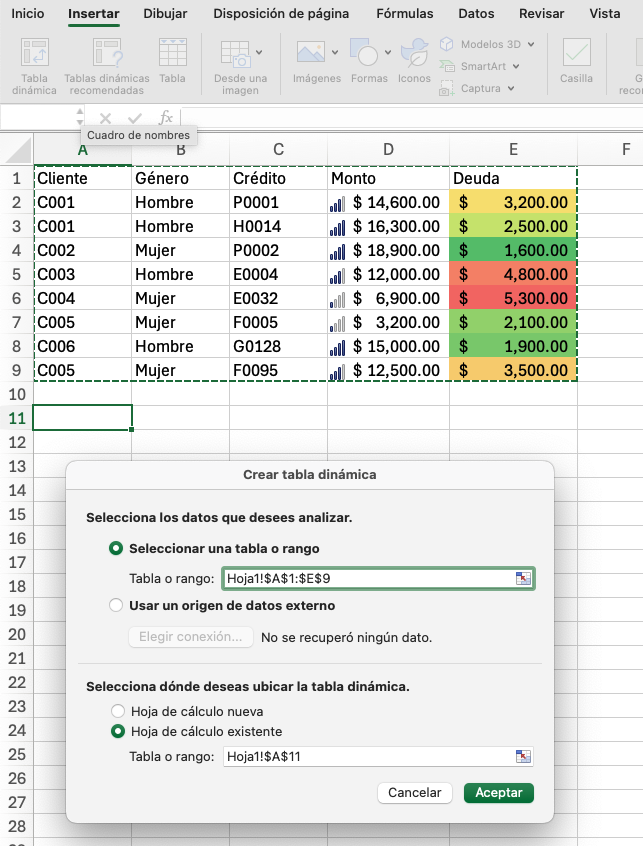
\includegraphics[width=\textwidth]{figures/s102-1.png}
    \end{minipage}
    \captionsetup{width=0.9\textwidth}
    \caption{Solución al Problema 2 inciso (a)}
    \label{fig:s102-1}
\end{figure}

\break
\noindent
Para el inciso (b) arrastramos los campos del género y cliente a las filas
\begin{figure}[!ht]
    \centering
    \begin{minipage}{\textwidth}
        \centering
        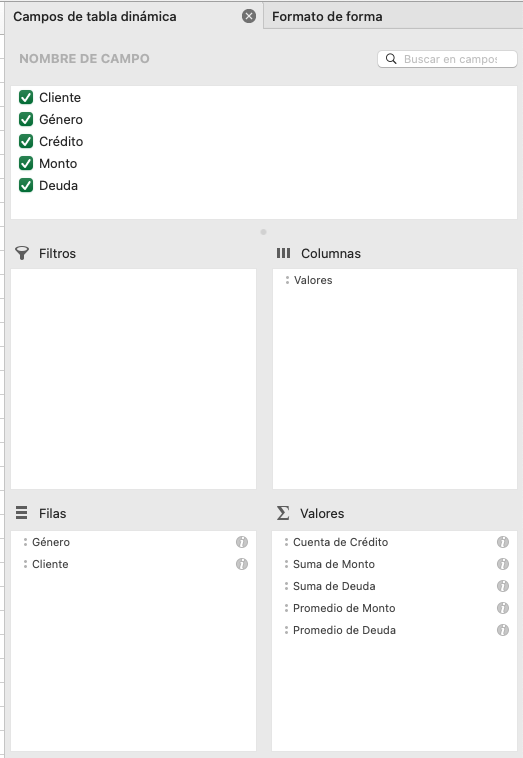
\includegraphics[width=\textwidth]{figures/s102-2.png}
    \end{minipage}
    \captionsetup{width=0.9\textwidth}
    \caption{Solución al Problema 2 inciso (b)}
    \label{fig:s102-2}
\end{figure}

\noindent
Para el inciso (c), (d), (e), (f), (g) arrastramos los campos como valores y configuramos cada campo si es recuento, suma o promedio
\begin{figure}[!ht]
    \centering
    \begin{minipage}{\textwidth}
        \centering
        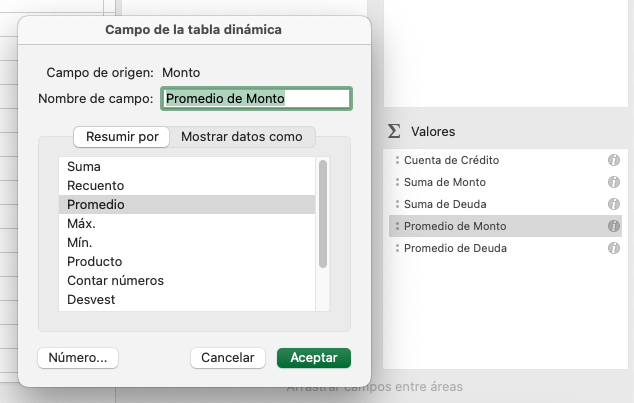
\includegraphics[width=\textwidth]{figures/s102-3.png}
    \end{minipage}
    \captionsetup{width=0.9\textwidth}
    \caption{Solución al Problema 2 incisos (c), (d), (e), (f), (g)}
    \label{fig:s102-3}
\end{figure}

\noindent
Para el inciso (h), (i), (j), (k), (l) observamos los valores en la tabla dinámica
\begin{figure}[!ht]
    \centering
    \begin{minipage}{\textwidth}
        \centering
        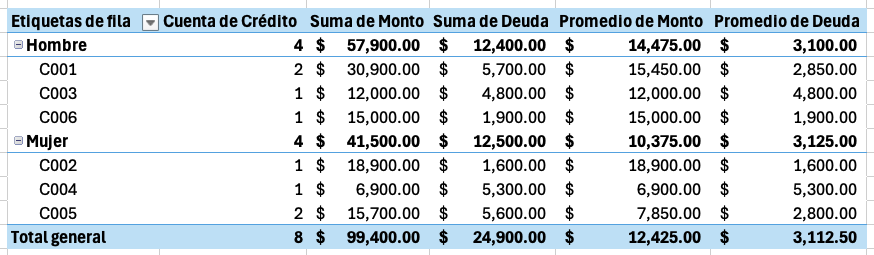
\includegraphics[width=\textwidth]{figures/s102-4.png}
    \end{minipage}
    \captionsetup{width=0.9\textwidth}
    \caption{Solución al Problema 2 incisos (h), (i), (j), (k), (l)}
    \label{fig:s102-4}
\end{figure}

\noindent
Respuestas: (h) \textbf{C001 \$5,700}, (i) \textbf{C002 \$18,900}, (j) \textbf{C003 \$4,800}, (k) \textbf{No, la diferencia es de \$100 menor al 1\% de diferencia}, (l) \textbf{\$74,500 = \$99,400 - \$24,900}.

\clearpage

\subsection*{Problema 3 | Uso de Power BI}

Una empresa financiera posee una tabla con los préstamos que ha aprobado a sus clientes indicando el monto, el estado y el valor. En cada préstamo se reporta el estado de sobre lo que se ha pagado del préstamo, lo que se debió haber cubierto actualmente (deuda) y lo que se debería cubrir en el futuro (pendiente). La financiera requiere una tabla que resuma de cada cliente sus préstamos y en cada préstamo se desglose la suma de cuánto adeuda, cuánto ha pagado y cuánto está pendiente, así como el total. También requiere un indicador que muestre la diferencia entre la suma del monto del préstamo y el valor del monto pagado, para saber cuánto se adeuda en total del préstamo, igualmente desglosado por cliente y préstamo. Finalmente la financiera requiere dos reportes visuales, un anillo que muestre el estado de los préstamos (pagado, pendiente y deuda) segmentado por cliente. Y un esquema jerárquico que permita desglosar el valor del préstamo por su estado, cliente y número de préstamo.
\\[12pt]
En la Figura \ref{fig:p103} se muestra la tabla de préstamos, con la columna del cliente, el número de préstamo, el monto, el estado (pagado, deuda, pendiente) y el valor asociado al estado.
\begin{figure}[!ht]
    \centering
    \begin{minipage}{\textwidth}
        \centering
        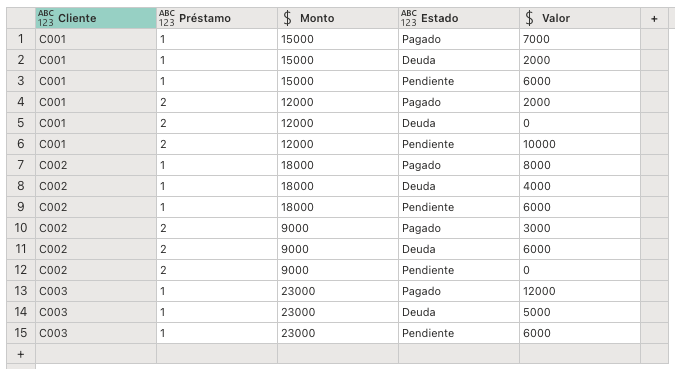
\includegraphics[width=\textwidth]{figures/p103.png}
    \end{minipage}
    \captionsetup{width=0.9\textwidth}
    \caption{Préstamos aprobados a clientes desglosado por cliente, número de préstamo, estado (pagado, deuda y pendiente) y valor asociado al estado}
    \label{fig:p103}
\end{figure}
\\

\break
\noindent
(a) Crea una matriz que reporte las filas para el cliente y número de préstamo en ese orden, el estado como columna y la suma del valor en los valores.
\\[6pt]
(b) En el modelo de datos crea una nueva medida con la fórmula
\\[6pt]
\texttt{Diferencia = SUM(P103[Monto])-SUM(P103[Valor])} 
\\[6pt]
para reportar la diferencia entre la suma del monto menos la suma del valor asociado al estado. Donde \textit{P103} es el nombre de la tabla creada al inicio.
\\[6pt]
(c) Crea una matriz que reporte las filas para el cliente y número de préstamo en ese orden, el estado como columna y la suma del monto, suma del valor y suma de diferencia en los valores en ese orden. Reporta solo el estado Pagado en los filtros del objeto visual.
\\[6pt]
(d) Crea una gráfica de anillo cuya leyenda este dada por el estado del préstamo, en valores reporte la suma del valor asociado al estado, y en detalles segmente al cliente.
\\[6pt]
(e) Crea un esquema jerárquico para analizar la suma del valor valor asociado al estado, explicado por el estado del préstamo, el cliente y el número de préstamo en ese orden.
\\[6pt]
(f) De la matriz del inciso (a) responde si cada desglose corresponde al monto reportado en cada préstamo.
\\[6pt]
(g) De la matriz del inciso (b) responde cuál el es el préstamo con menor deuda total y usando el inciso (a) cómo es su deuda respecto al préstamo.
\\[6pt]
(h) Del anillo identifica al cliente de mayor deuda y el cliente con mayor valor pendiente.
\\[6pt]
(i) Del esquema jerárquico identifica al cliente de mayor deuda y el número de préstamo de mayor deuda para ese cliente.

\clearpage

\subsubsection*{Solución al Problema 3}

Para el inciso (a) creamos una matriz que reporte las filas para el cliente y número de préstamo en ese orden, el estado como columna y la suma del valor en los valores.
\begin{figure}[!ht]
    \centering
    \begin{minipage}{\textwidth}
        \centering
        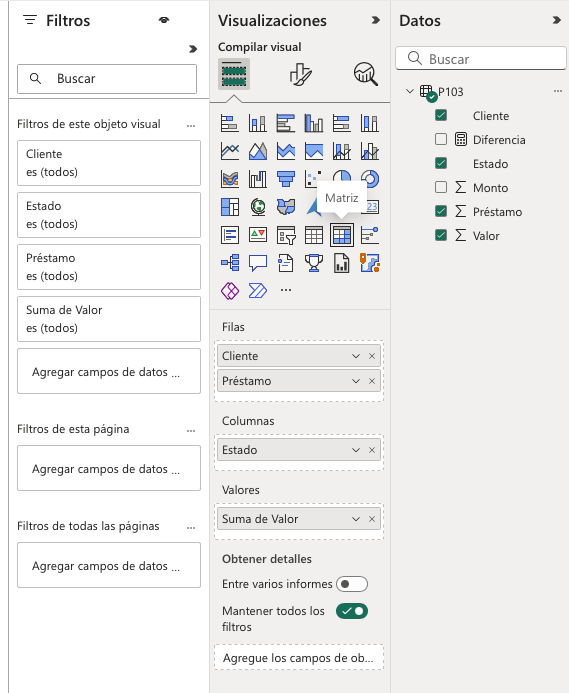
\includegraphics[width=0.7\textwidth]{figures/s103a-1.png}
    \end{minipage}
    \hfill
    \begin{minipage}{\textwidth}
        \centering
        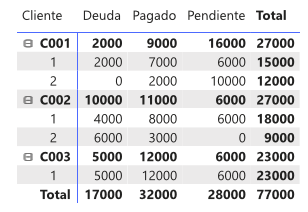
\includegraphics[width=0.7\textwidth]{figures/s103a-2.png}
    \end{minipage}
    \captionsetup{width=0.9\textwidth}
    \caption{Solución al Problema 3 inciso (a)}
    \label{fig:s103a}
\end{figure}

\noindent
Para el inciso (b) abrimos el modelo de datos y dentro del modelo de datos creamos una nueva medida con la fórmula para calcular la diferencia.
\begin{figure}[!ht]
    \centering
    \begin{minipage}{\textwidth}
        \centering
        
\includegraphics[width=\textwidth]{figures/s103b-1.png}
    \end{minipage}
    \hfill
    \begin{minipage}{\textwidth}
        \centering
        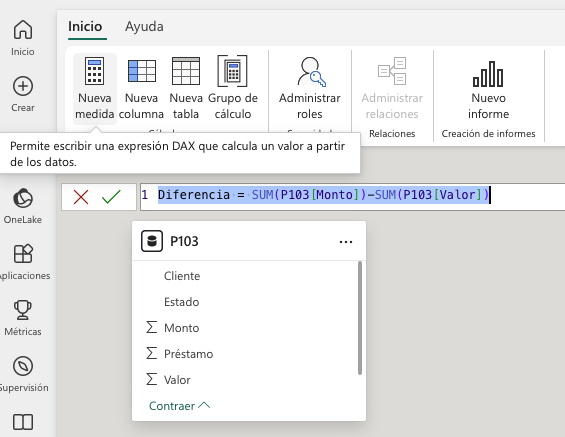
\includegraphics[width=\textwidth]{figures/s103b-2.png}
    \end{minipage}
    \hfill
    \begin{minipage}{\textwidth}
        \centering
        
\includegraphics[width=\textwidth]{figures/s103b-3.png}
    \end{minipage}
    \captionsetup{width=0.9\textwidth}
    \caption{Solución al Problema 3 inciso (b)}
    \label{fig:s103b}
\end{figure}

\break
\noindent
Para el inciso (c) creamos una matriz que reporte las filas para el cliente y número de préstamo en ese orden, el estado como columna y la suma del monto, suma del valor y suma de diferencia en los valores en ese orden. Reporta solo el estado Pagado en los filtros del objeto visual.
\begin{figure}[!ht]
    \centering
    \begin{minipage}{\textwidth}
        \centering
        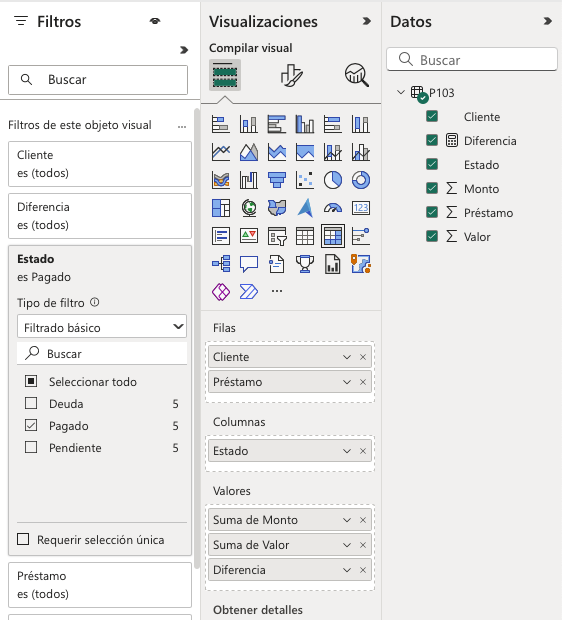
\includegraphics[width=0.9\textwidth]{figures/s103c-1.png}
    \end{minipage}
    \hfill
    \begin{minipage}{\textwidth}
        \centering
        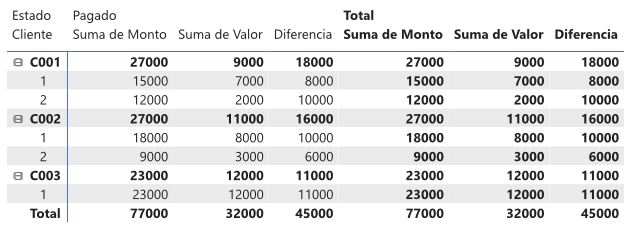
\includegraphics[width=0.9\textwidth]{figures/s103c-2.png}
    \end{minipage}
    \captionsetup{width=0.9\textwidth}
    \caption{Solución al Problema 3 inciso (c)}
    \label{fig:s103c}
\end{figure}

\noindent
Para el inciso (d) creamos una gráfica de anillo cuya leyenda este dada por el estado del préstamo, en valores reporte la suma del valor asociado al estado, y en detalles segmente al cliente.
\begin{figure}[!ht]
    \centering
    \begin{minipage}{\textwidth}
        \centering
        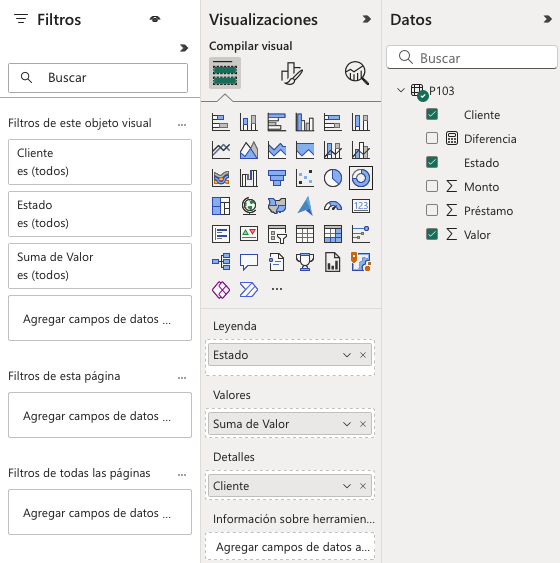
\includegraphics[width=0.8\textwidth]{figures/s103d-1.png}
    \end{minipage}
    \hfill
    \begin{minipage}{\textwidth}
        \centering
        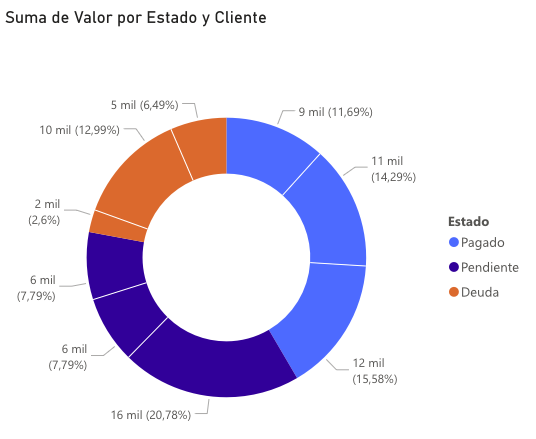
\includegraphics[width=0.7\textwidth]{figures/s103d-2.png}
    \end{minipage}
    \captionsetup{width=0.9\textwidth}
    \caption{Solución al Problema 3 inciso (d)}
    \label{fig:s103d}
\end{figure}

\noindent
Para el inciso (e) creamos un esquema jerárquico para analizar la suma del valor valor asociado al estado, explicado por el estado del préstamo, el cliente y el número de préstamo en ese orden.
\begin{figure}[!ht]
    \centering
    \begin{minipage}{\textwidth}
        \centering
        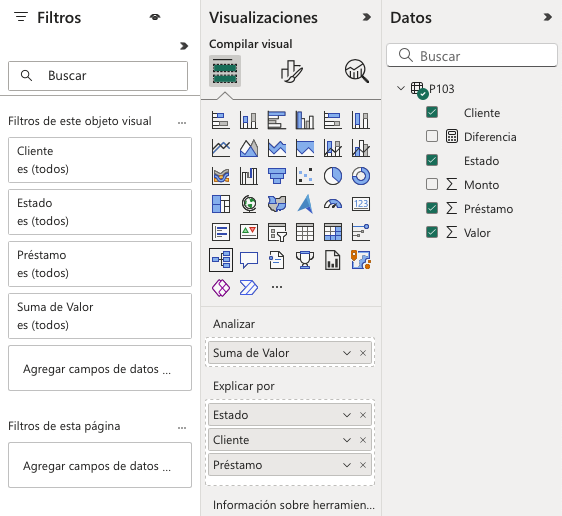
\includegraphics[width=0.9\textwidth]{figures/s103e-1.png}
    \end{minipage}
    \hfill
    \begin{minipage}{\textwidth}
        \centering
        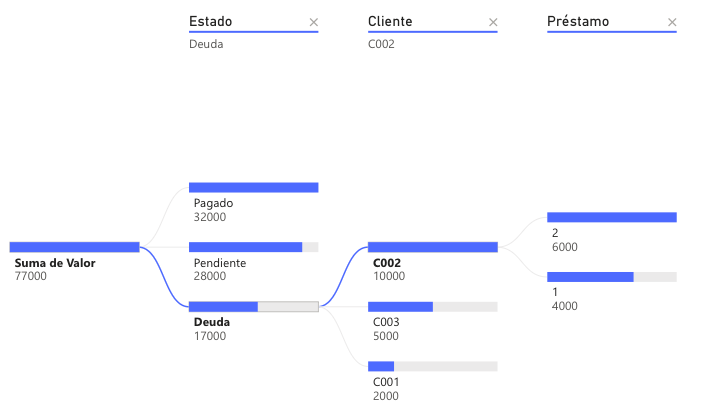
\includegraphics[width=0.9\textwidth]{figures/s103e-2.png}
    \end{minipage}
    \captionsetup{width=0.9\textwidth}
    \caption{Solución al Problema 3 inciso (e)}
    \label{fig:s103e}
\end{figure}

\noindent
Para los otros incisos las respuestas son: (f) Sí, la suma de montos en cada préstamo coincide con la suma de su deuda, lo pagado y lo pendiente. (g) Para el cliente \textit{C002} en el préstamo número \textit{2} la diferencia total es de \textbf{\$6,000} y es el préstamo de menor deuda, ya que lo pendiente para ese préstamo es de \textbf{\$0}, sin embargo, respecto a los otros préstamos es el de mayor deuda. (h) \textbf{C002 \$10,000 12.99\%} es el cliente de mayor deuda y \textbf{C001 \$16,000 20.78\%} es el cliente de mayor valor pendiente. (i) \textbf{C002 \$10,000 2 \$10,000} es el cliente de mayor deuda, con su préstamo número dos.

\clearpage

\subsection*{Problema 4 | Uso de Python}

Un banco ha decidido usar Python en un ambiente controlado para poder hacer operaciones y cálculos de riesgo, para ello ha instalado un ambiente virtual cerrado en computadoras sin acceso a internet para que no se filtren los conjuntos de datos utilizados, ni los reportes generados.
\\[12pt]
El banco comenzará por automatizar una serie de funciones útiles que pueda aplicar para cálculos simples, para de esta forma crear una metodología de trabajo cuando deseen incrementar el volumen de las operaciones.
\\[12pt]
Para ello, el banco requiere que se generen los siguientes reportes automatizados para saber que todo está funcionando correctamente.
\\[12pt]
Implementa las funciones que se detallan a continuación y resuelve los incisos siguietes. Completa el código que haga falta para que las funciones operen correctamente siguiendo las pistas de los comentarios
\scriptsize
\begin{verbatim}
def reporteTitulo(codigo, leyenda):
    print(f"Banco Nacional - Reporte {codigo} / {leyenda}")

def reporteCorte(codigo, leyenda):
    print(f"-------------- {codigo} / {leyenda} --------------")

def reporteFin(codigo, leyenda):
    print(f"-------------- {codigo} / {leyenda} --------------")

def reporteBalanceDiaInicio(balance):
    reporteTitulo("BIN", "Balance al Inicio del Día")
    print(f"$ {balance:.2f}")
    reporteFin("BIN", "Balance al Inicio del Día")

def reporteBalanceDiaFin(balance):
    reporteTitulo("B-OUT", "Balance al Final del Día")
    print(f"$ {balance:.2f}")
    reporteFin("B-OUT", "Balance al Final del Día")

def reporteTotalOperacionesDia(numOperaciones):
    reporteTitulo("T-OP", "Total de Operaciones del Día")
    # Imprime el número de operaciones
    reporteFin("T-OP", "Total de Operaciones del Día")

def reporteTotalOperacionesRelativasMes(numOperacionesDia, numOperacionesMes):
    reporteTitulo("T-OR", "Tasa de Operaciones del día respecto al mes")
    tasa = 100 * numOperacionesDia / numOperacionesMes
    # Imprime el número de operaciones del dia
    # luego una diagonal y el número de operaciones del mes
    # Haz un corte del reporte
    # Imprime la tasa de operaciones del día respecto al mes a un dígito
    # Ejemplo: 41/200 (20.5%)
    reporteFin("T-OR", "Tasa de Operaciones del día respecto al mes")
\end{verbatim}
\hfill
\normalsize

\noindent
(a) Reporta el balance de inicio del día con \textbf{\$ 185,000.32}
\\[6pt]
(b) Reporta un total de \textbf{247} operaciones del día
\\[6pt]
(c) Reporta un total de \textbf{247} de \textbf{192,316} operaciones relativas del mes
\\[6pt]
(d) Reporta el balance de fin del día con \textbf{\$ 232,827.71}
\\[6pt]

\subsection*{Problema 5 | Interés Simple}

Una financiera posee montos de préstamos a proyectos y la tasa anual fija que le cobrará sus clientes. La financiera requiere calcular la suma de montos y proponer una misma tasa de interés anual única para todos los proyectos, así como encontrar la tasa anual en caso de perder el monto por algún proyecto.
\\[12pt]
En la Figura \ref{fig:p105} se muestran los montos y la tasa anual de los montos de préstamo destinados a proyectos financiados.
\begin{figure}[!ht]
    \centering
    \begin{minipage}{\textwidth}
        \centering
        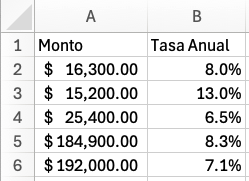
\includegraphics[width=\textwidth]{figures/p105.png}
    \end{minipage}
    \captionsetup{width=0.9\textwidth}
    \caption{Montos de préstamos a proyectos de una financiera y su tasa anual}
    \label{fig:p105}
\end{figure}
\\

\noindent
(a) Calcula el interés simple generado por la tasa anual y reporta cada interés y la suma de todos estos intereses. 
\\[6pt]
(b) Calcula la tasa anual promedio y de todas las tasas y la suma de todos los montos y calcula el interés de la suma total con la tasa anual promedio. ¿Este interés es el mismo que el del la suma del inciso (a)?
\\[6pt]
(c) ¿Cuál debería ser la tasa anual de todos los montos para que la suma del interés sea la misma?
\\[6pt]
(d) ¿Cuál debería ser la tasa anual de todos los montos, si no existiera el monto de \textbf{\$ 25,400.00} para que la suma del interés sea la misma a las anteriores?

\subsection*{Problema 6 | Interés Compuesto}

Una financiera desea calcular el interés compuesto que generaría un monto de \textbf{\$ 4,312,939.83} con una tasa anual de \textbf{8\%}, si se tuviera que pagar mensualmente a una tasa compuesta de \textbf{0.67\%} y si tuviera que pagar a tasa compuesta de \textbf{0.34\%}.
\\[12pt]
(a) Calcula el interés compuesto a 12 meses con una tasa mensual de \textbf{0.67\%}. 
\\[6pt]
(b) Calcula el interés compuesto a 24 quincenas con una tasa quincenal de \textbf{0.34\%}

\clearpage

\subsection*{Problema 7 | Tasa de Interés Variable}

Una financiera desea calcular el interés que generaría un monto de \textbf{\$ 2,617,800.01} con una tasa mensual variable que comienza en \textbf{6\%} el primer mes y se actualiza a \textbf{5\%} para el segundo mes, luego \textbf{4\%} al tercer mes, \textbf{3\%} para el cuarto mes y luego \textbf{2\%} y \textbf{1\%} para el quinto y sexto mes, luego de ahí se aplica el \textbf{0.5\%} en los meses restantes.
\\[12pt]
(a) Calcula el interés compuesto para los 12 meses usando el interés variable. 
\\[6pt]
(b) Si se usara un interés anual fijo, ¿De cuánto sería?

\clearpage

\subsection*{Problema 8 | Tabla de Amortización Simple}

Una financiera desea calcular una tabla de amortización para un monto financiado de \textbf{\$ 6,500.00}, con un enganche inicial de \textbf{\$ 2,300.00}, el cual pagará los intereses amortizados. Los intereses están diseñados para que bajen linealmente durante 48 semanas y recuperen \textbf{80\%} del monto financiado. Es decir, se necesitan recuperar intereses por el \textbf{80\%} de los \textbf{\$ 6,500.00}, diseñando intereses que se reduzcan linealmente en 48 pagos y luego se considere el enganche inicial como descuento inmediato a los primeros intereses.
\\[12pt]
(a) Calcula la tabla de amortización sin considerar el enganche.
\\[6pt]
(b) ¿Cuántos pagos iniciales cubre el enganche?
\\[6pt]
(c) Determina un abono fijo para terminar de pagar los intereses más el monto financiado en 48 semanas.

\clearpage

\subsection*{Problema 9 | Interés Simple Futuro}

Un banco financió un proyecto durante 36 meses por \textbf{\$ 8,496,500.00}, con una tasa anual fija y simple del \textbf{12\%} y desea calcular los intereses que se generarán al mes 25 y al mes 30. También desea saber en qué mes los intereses superarán el valor de los \textbf{\$ 40,000.00}.
\\[12pt]
(a) Calcula los intereses para el mes 25 y 30.
\\[6pt]
(b) Determina en qué mes los intereses superarán los \textbf{\$ 40,000.00}.
\\[6pt]
(c) Calcula el valor de las cuotas fijas para cubrir el préstamos en los 36 meses.
\\[6pt]
(d) Calcula el valor de las cuotas fijas para cubrir el préstamos en los 36 meses, si se da un adelanto del \textbf{10\%} del valor del proyecto (los intereses deberían ser los mismos).

\clearpage

\subsection*{Problema 10 | Punto de Liquidación}

Un banco financió un proyecto durante 48 meses por \textbf{\$ 6,232,800.00}, con una tasa anual fija y simple del \textbf{12\%} y desea calcular el valor de liquidación que considere pagar los intereses futuros y la deuda total, la liquidación se llevará a cabo en el mes 28.
\\[12pt]
(a) Calcula los intereses totales.
\\[6pt]
(b) Calcula los intereses faltantes a partir del mes 28.
\\[6pt]
(c) Calcula la deuda de liquidación para el mes 28.

\clearpage

\section*{Módulo II | Estadística y Probabilidad con Python}

\subsection*{Problema 1 | Probabilidad de un Evento Simple} 

Una financiera posee una tabla con el género de sus clientes, si tiene trabajo, si está casado y si tiene alguna deuda.
\\[12pt]
En la Figura \ref{fig:p201} se muestra la tabla con el género, trabajo, casado y deuda de los clientes.
\begin{figure}[!ht]
    \centering
    \begin{minipage}{\textwidth}
        \centering
        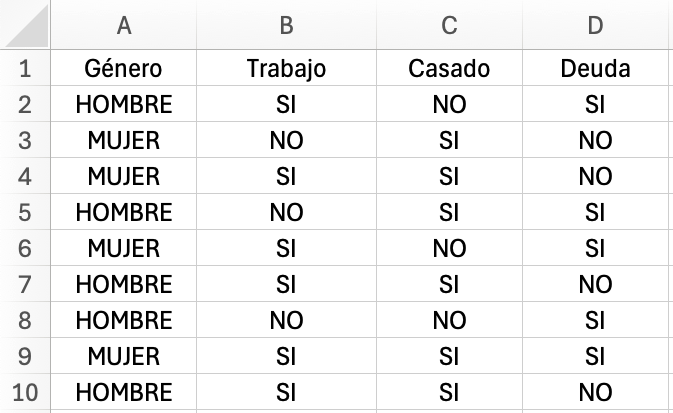
\includegraphics[width=\textwidth]{figures/p201.png}
    \end{minipage}
    \captionsetup{width=0.9\textwidth}
    \caption{Tabla de deuda por género, trabajo y casado}
    \label{fig:p201}
\end{figure}
\\
(a) Calcula la probabilidad de ser hombre
\\[6pt]
(b) Calcula la probabilidad de ser mujer
\\[6pt]
(c) Calcula la probabilidad de tener trabajo
\\[6pt]
(d) Calcula la probabilidad de no tener trabajo
\\[6pt]
(e) Calcula la probabilidad de estar casado
\\[6pt]
(f) Calcula la probabilidad de no estar casado
\\[6pt]
(g) Calcula la probabilidad de tener deuda
\\[6pt]
(h) Calcula la probabilidad de no tener deuda

\clearpage

\subsection*{Problema 2 | Tabla conjunta de Dos Eventos}

Un restaurante está inspeccionando la bebidas asociadas al pago con tarjeta de sus clientes, porque sospecha que los clientes que pagan con tarjeta de crédito consumen más cerveza que aquellos que pagan con tarjeta de débito.
\\[12pt]
En la Figura \ref{fig:p202} se muestra la tabla con los datos de los clientes si utilizaron tarjeta de crédito o débito y el tipo de bebida que consumieron.
\begin{figure}[!ht]
    \centering
    \begin{minipage}{\textwidth}
        \centering
        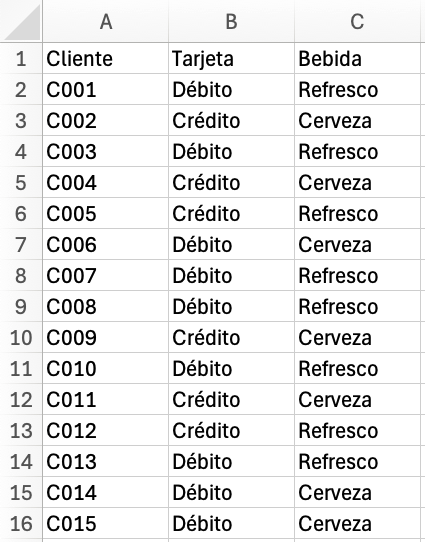
\includegraphics[width=0.9\textwidth]{figures/p202.png}
    \end{minipage}
    \captionsetup{width=0.9\textwidth}
    \caption{Tabla de tipo bebida consumida asociada al tipo de tarjeta}
    \label{fig:p202}
\end{figure}
\\

\break
\noindent
(a) Genera la tabla conjunta donde las filas sean el tipo de tarjeta (Débito, Crédito) y las columnas el tipo de bebida (Refresco, Cerveza). En cada celda pon el número total de registros que cumplen la fila y la columna, por ejemplo, para la fila Débito y la columna Refresco, hay 6 registros.
\\[6pt]
(b) Agrega una columna adicional con los totales marginales para la fila, sumando todas las columnas.
\\[6pt]
(c) Agrega una fila adicional para los totales marginales para la columna, sumando todas las filas.
\\[6pt]
(d) Indica el total de registros en la intersección de la columna marginal y la fila marginal.
\\[6pt]
(e) Genera la tabla de probabilidad conjunta, que es la misma que la tabla conjunta, solo que cada valor está dividido sobre el total de registros.
\\[6pt]
(f) Calcula la probabilidad de tener una tarjeta de débito
\\[6pt]
(g) Calcula la probabilidad de tener una tarjeta de crédito
\\[6pt]
(h) Calcula la probabilidad de haber consumido refresco
\\[6pt]
(i) Calcula la probabilidad de tener consumido cerveza

\clearpage

\subsection*{Problema 3 | Probabilidad Conjunta de Dos Eventos}

Una empresa ha recuperado la tabla conjunta del personal que fue promovido a un mejor puesto y los que no a lo largo de 3 años. La tabla divide los hombres y mujeres contra si fueron o no promovidos, también cuenta con sus totales marginales. La empresa necesita encontrar la probabilidad conjunta de que los hombres hayan sido promividos o no.
\\[12pt]
En la Figura \ref{fig:p203} se muestra la tabla conjunta de promoción del personal por género.
\begin{figure}[!ht]
    \centering
    \begin{minipage}{\textwidth}
        \centering
        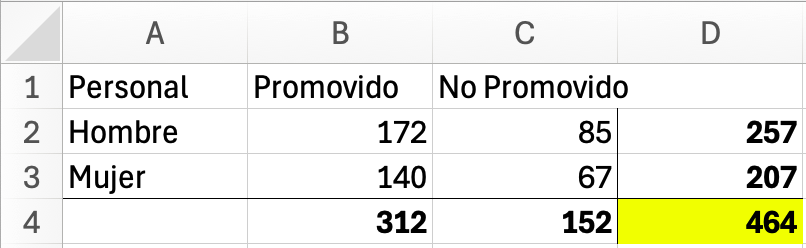
\includegraphics[width=\textwidth]{figures/p203.png}
    \end{minipage}
    \captionsetup{width=0.9\textwidth}
    \caption{Tabla conjunta de promoción del personal por género}
    \label{fig:p203}
\end{figure}
\\
(a) Divide cada valor de la tabla conjunta por el total marginal de $464$.
\\[6pt]
(b) Indica cual es la probabilidad total de que un hombre haya sido promovido.
\\[6pt]
(c) Indica cual es la probabilidad total de que un hombre no haya sido promovido.
\\[6pt]
(d) Indica cual es la probabilidad total de que una mujer haya sido promovida.
\\[6pt]
(e) Indica cual es la probabilidad total de que una mujer no haya sido promovida.
\\[6pt]
(f) Indica cual es la probabilidad total de que alguien sea hombre.
\\[6pt]
(g) Indica cual es la probabilidad total de que alguien sea mujer.
\\[6pt]
(h) Indica cual es la probabilidad total de que alguien sea promovido.
\\[6pt]
(i) Indica cual es la probabilidad total de que alguien no sea promovido.

\clearpage

\subsection*{Problema 4 | Probabilidad Condicional de Dos Eventos}

Una fábrica de cosméticos está diseñando un nuevo programa para que sus empleados trabajen dos horas menos de lo convencional. Para determinar si su modelo funciona, ha contratado empleados temporales, a los cuales se les pregunta si quieren ganar \textbf{\$ 2,800} por 6 horas diarias durante los 6 días de jornada de la semana, o ganar \textbf{\$ 4,080} por 8 horas. Al cabo de la semana, el empleado temporal tiene la oportunidad de tener un contrato de 3 meses o renunciar.
\\[12pt]
Después de construir la tabla conjunta con el número de empleados que trabajaron 6 horas u 8 horas y que renunciaron o no renunciaron, la empresa decide generar la tabla de probabilidad conjunta para no exponer los números netos sobre los empleados que contrató. Ahora requiere calcular la probabilidad de haber trabajado 6 horas dado que renunció y haber trabajado 8 horas dado que renunció, para poder entender cuál era turno que eligió una persona que decidió renunciar al final.
\\[12pt]
Además la empresa necesita saber cuál es la probabilidad de renunciar, dado que se trabaja 6 horas y la probabilidad de renunciar dado que se trabaja 8 horas, para entender quién tiene mayor probabilidad de renunciar y decidir si vale la pena mantener un turno de 8 horas en el futuro.
\\[12pt]
En la Figura \ref{fig:p204} se muestra la tabla de probabilidad de los empleados que deciden renunciar o no en turnos de 6 y 8 horas.
\begin{figure}[!ht]
    \centering
    \begin{minipage}{\textwidth}
        \centering
        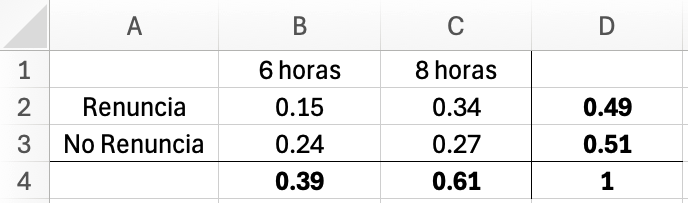
\includegraphics[width=\textwidth]{figures/p204.png}
    \end{minipage}
    \captionsetup{width=0.9\textwidth}
    \caption{Tabla de probabilidad de renuncia por turno}
    \label{fig:p204}
\end{figure}
\\

\break
\noindent
(a) Indica cual es la probabilidad que alguien renuncie $P(Renuncia)$
\\[6pt]
(b) Indica la probabilidad de que alguien trabaje 6 horas $P(6h)$
\\[6pt]
(c) Indica la probabilidad de que alguien trabaje 8 horas $P(8h)$
\\[6pt]
(d) Indica la probabilidad de que alguien trabaje trabaje 6 horas y renuncie $P(6h \cap Renuncia)$
\\[6pt]
(e) Indica la probabilidad de que alguien trabaje trabaje 8 horas y renuncie $P(8h \cap Renuncia)$
\\[6pt]
(f) Calcula la probabilidad de trabajar 6 horas dado que se renuncia 
\\[6pt]
$P(6h|Renuncia) = \frac{P(6h \cap Renuncia)}{P(Renuncia)}$.
\\[6pt]
(g) Calcula la probabilidad de trabajar 8 horas dado que se renuncia
\\[6pt]
$P(8h|Renuncia) = \frac{P(8h \cap Renuncia)}{P(Renuncia)}$.
\\[6pt]
(h) Calcula la probabilidad de renunciar dado que se trabajó 6 horas 
\\[6pt]
$P(Renuncia|6h) = \frac{P(6h \cap Renuncia)}{P(6h)}$.
\\[6pt]
(i) Calcula la probabilidad de renunciar dado que se trabajó 6 horas 
\\[6pt]
$P(Renuncia|8h) = \frac{P(8h \cap Renuncia)}{P(8h)}$.

\clearpage

\subsection*{Problema 5 | Probabilidad Conjunta de Tres Eventos}

\subsection*{Problema 6 | Probabilidad Condicional de Tres Eventos}

\subsection*{Problema 7 | Estadísticos Principales de Un Eje}

\subsection*{Problema 8 | Estadísticos Principales de Dos Ejes }

\subsection*{Problema 9 | Matriz de Correlación entre Tres Ejes}

\subsection*{Problema 10 | Prueba F entre Dos Hipótesis de Un Eje}

\clearpage

\section*{Módulo III | Ciencia de Datos}

\subsection*{Problema 1 | Estructuración de un Dataset en Excel}

Crea un archivo Excel que represente la siguiente información:

\begin{table}[h]
    \centering
    \begin{tabular}{|c|c|c|c|}
        \hline
        País & Año & Población (millones) & PIB per cápita (USD) \\
        \hline
        México & 2022 & 126 & 10000 \\
        Estados Unidos & 2022 & 331 & 63000 \\
        Canadá & 2022 & 38 & 48000 \\
        Brasil & 2022 & 213 & 7500 \\
        Japón & 2022 & 126 & 40000 \\
        \hline
    \end{tabular}
    \caption{Datos para estructurar}
\end{table}

Guarda el archivo con el nombre \texttt{indicadores.xlsx}.

\clearpage

\subsection*{Problema 2 | Dataset de indicadores en CSV}

Convierte el archivo \texttt{indicadores.xlsx} del Problema 1 en un archivo CSV llamado \texttt{indicadores.csv}. Usa el siguiente formato de columnas:

\begin{verbatim}
País,Año,Población,PIB_per_capita
México,2022,126,10000
Estados Unidos,2022,331,63000
Canadá,2022,38,48000
Brasil,2022,213,7500
Japón,2022,126,40000
\end{verbatim}

\clearpage

\subsection*{Problema 3 | Adquisición de un CSV en Python}

Escribe un script en Python que lea el archivo \texttt{indicadores.csv} del Problema 2 y lo muestre en la consola. Completa el siguiente código:

\begin{lstlisting}[style=python]
import pandas as pd

# Ruta del archivo
file_path = "..."

# Cargar el CSV
df = pd.read_csv(file_path)

# Mostrar el DataFrame
print(...)
\end{lstlisting}

\clearpage

\subsection*{Problema 4 | Indicadores en Series de Pandas}

Usando el DataFrame cargado en el Problema 3, crea una Serie con los valores del PIB per cápita. Completa el siguiente código:

\begin{lstlisting}[style=python]
# Crear la Serie
pib_per_capita = ...

# Mostrar la Serie
print(pib_per_capita)
\end{lstlisting}

\clearpage

\subsection*{Problema 5 | Indicadores en DataFrames de Pandas}

Agrega una nueva columna llamada \texttt{PIB\_total} que calcule el PIB total como el producto de \texttt{Población} y \texttt{PIB per cápita}. Completa el código:

\begin{lstlisting}[style=python]
# Agregar la columna
df['PIB_total'] = ...

# Mostrar el DataFrame
print(df)
\end{lstlisting}

\clearpage

\subsection*{Problema 6 | Filtrar columnas en DataFrames}

Filtra únicamente las columnas \texttt{País} y \texttt{PIB\_total}. Completa el código:

\begin{lstlisting}[style=python]
# Filtrar columnas
filtered_df = df[...]

# Mostrar las columnas filtradas
print(filtered_df)
\end{lstlisting}

\clearpage

\subsection*{Problema 7 | Filtrar filas en DataFrames}

Filtra las filas donde el PIB total sea mayor a 1 billón de USD (\texttt{1e12}). Completa el código:

\begin{lstlisting}[style=python]
# Filtrar filas
high_pib = df[...]

# Mostrar las filas filtradas
print(high_pib)
\end{lstlisting}

\clearpage

\subsection*{Problema 8 | Agrupación de datos en DataFrames}

Agrupa los datos por año y calcula el promedio de PIB per cápita. Completa el código:

\begin{lstlisting}[style=python]
# Agrupar y calcular promedio
average_pib = df.groupby(...)[...].mean()

# Mostrar el resultado
print(average_pib)
\end{lstlisting}

\clearpage

\subsection*{Problema 9 | Combinación de datos en DataFrames}

Combina el DataFrame actual con otro que contenga información adicional, como índice de desarrollo humano (IDH). Completa el código:

\begin{lstlisting}[style=python]
# Crear otro DataFrame
idh_data = {
    "Pais": ["Mexico", "Estados Unidos", "Canada", "Brasil", "Japon"],
    "IDH": [0.758, 0.926, 0.929, 0.765, 0.919]
}
idh_df = pd.DataFrame(idh_data)

# Combinar DataFrames
combined_df = pd.merge(df, idh_df, on=...)

# Mostrar el resultado
print(combined_df)
\end{lstlisting}

\clearpage

\subsection*{Problema 10 | Visualización de datos}

Crea un gráfico de barras que muestre el PIB total por país usando la librería \texttt{matplotlib}. Completa el código:

\begin{lstlisting}[style=python]
import matplotlib.pyplot as plt

# Crear grafico de barras
plt.bar(..., ...)

# Configurar etiquetas
plt.xlabel("Pais")
plt.ylabel("PIB Total (USD)")
plt.title("PIB Total por Pais")

# Mostrar grafico
plt.show()
\end{lstlisting}

\section*{Módulo IV | Machine Learning}


% Problema 1
\subsection*{Problema 1 | Aprendizaje Supervisado}

Dado el siguiente conjunto de datos en formato CSV:

\begin{verbatim}
Edad,Salario,Compra
25,50000,No
35,60000,Sí
45,80000,Sí
30,70000,No
40,85000,Sí
\end{verbatim}

Carga estos datos en un DataFrame de pandas y utiliza la librería \texttt{sklearn} para entrenar un modelo de clasificación que prediga si una persona comprará un producto basado en su edad y salario.

\begin{lstlisting}[style=python]
from sklearn.model_selection import train_test_split
from sklearn.tree import DecisionTreeClassifier
import pandas as pd

# Cargar los datos
data = ...

# Separar variables independientes y dependientes
X = ...
y = ...

# Dividir los datos en conjuntos de entrenamiento y prueba
X_train, X_test, y_train, y_test = train_test_split(...)

# Entrenar el modelo
model = DecisionTreeClassifier()
model.fit(...)

# Evaluar el modelo
accuracy = model.score(...)
print(f"Accuracy: {accuracy}")
\end{lstlisting}

\clearpage

% Problema 2
\subsection*{Problema 2 | Regresión Simple}

Usa el siguiente conjunto de datos para predecir el precio de una casa basado en su tamaño en pies cuadrados:

\begin{verbatim}
Tamaño,Precio
1000,150000
1500,200000
2000,250000
2500,300000
3000,350000
\end{verbatim}

Crea un modelo de regresión lineal y muestra la ecuación de la recta ajustada.

\begin{lstlisting}[style=python]
from sklearn.linear_model import LinearRegression

# Datos
X = ...
y = ...

# Crear modelo
model = LinearRegression()
model.fit(...)

# Mostrar ecuacion de la recta
print(f"Coeficiente: {model.coef_}")
print(f"Intercepto: {model.intercept_}")
\end{lstlisting}

\clearpage

% Problema 3
\subsection*{Problema 3 | Regresión Múltiple}

Amplía los datos del Problema 2 agregando una columna de número de habitaciones:

\begin{verbatim}
Tamaño,Habitaciones,Precio
1000,2,150000
1500,3,200000
2000,4,250000
2500,4,300000
3000,5,350000
\end{verbatim}

Entrena un modelo de regresión múltiple para predecir el precio de una casa.

\clearpage

% Problema 4
\subsection*{Problema 4 | Clasificación Simple}

Utilizando el conjunto de datos del Problema 1, usa una regresión logística para predecir la compra de un producto.

\begin{lstlisting}[style=python]
from sklearn.linear_model import LogisticRegression

# Crear modelo
model = LogisticRegression()
model.fit(...)

# Prediccion
pred = model.predict(...)
print(f"Predicciones: {pred}")
\end{lstlisting}

\clearpage

% Problema 5
\subsection*{Problema 5 | Clasificación Múltiple}

Dado el siguiente conjunto de datos, crea un modelo de clasificación que prediga la categoría del cliente (A, B o C) basado en el ingreso y la edad:

\begin{verbatim}
Edad,Ingreso,Categoría
25,30000,A
35,50000,B
45,70000,C
30,40000,A
40,60000,B
\end{verbatim}

\clearpage

% Problema 6
\subsection*{Problema 6 | Aprendizaje No Supervisado}

Usa el siguiente conjunto de datos para aplicar el algoritmo de K-Means y agrupar los puntos en 2 clústeres:

\begin{verbatim}
X,Y
1,2
2,1
3,4
5,6
6,5
\end{verbatim}

\begin{lstlisting}[style=python]
from sklearn.cluster import KMeans

# Datos
X = ...

# Crear modelo
kmeans = KMeans(n_clusters=2)
kmeans.fit(...)

# Mostrar centroides
print(f"Centroides: {kmeans.cluster_centers_}")
\end{lstlisting}

\clearpage

% Problema 7
\subsection*{Problema 7 | Reducción de Dimensionalidad}

Aplica PCA (Análisis de Componentes Principales) a un dataset con 3 dimensiones y reduce el espacio a 2 dimensiones. Usa datos sintéticos generados con \texttt{numpy}.

\clearpage

% Problema 8
\subsection*{Problema 8 | Matriz de Adyacencia}

Crea una matriz de adyacencia que represente el siguiente grafo:

\[
A \leftrightarrow B, \; A \leftrightarrow C, \; B \leftrightarrow D, \; C \leftrightarrow D
\]

\begin{lstlisting}[style=python]
import numpy as np

# Matriz de adyacencia
adj_matrix = np.array([
    [0, 1, 1, 0],
    [1, 0, 0, 1],
    [1, 0, 0, 1],
    [0, 1, 1, 0]
])

print(adj_matrix)
\end{lstlisting}

\clearpage

% Problema 9
\subsection*{Problema 9 | Matriz de Similitud}

Dado un conjunto de puntos en un espacio 2D, calcula una matriz de similitud basada en la distancia euclidiana inversa.

\clearpage

% Problema 10
\subsection*{Problema 10 | Clusterización}

Aplica el algoritmo DBSCAN para encontrar clústeres en el siguiente conjunto de datos:

\begin{verbatim}
X,Y
1,2
2,2
3,3
8,8
8,9
25,30
\end{verbatim}

\begin{lstlisting}[style=python]
from sklearn.cluster import DBSCAN

# Datos
X = ...

# Aplicar DBSCAN
dbscan = DBSCAN(eps=2, min_samples=2)
dbscan.fit(...)

# Mostrar etiquetas de cluster
print(f"Etiquetas: {dbscan.labels_}")
\end{lstlisting}

\clearpage

\section*{Módulo IV | Deep Learning}

% Problema 1
\subsection*{Problema 1 | Modelo Generalizado}

Construye un modelo generalizado con Keras que tenga:

- Una capa de entrada con 10 neuronas.
- Una capa oculta con 16 neuronas y activación ReLU.
- Una capa de salida con una sola neurona y activación sigmoidal.

\begin{lstlisting}[style=python]
from keras.models import Sequential
from keras.layers import Dense

# Crear el modelo
model = Sequential([
    Dense(16, activation='relu', input_shape=(10,)),
    ...
])

# Compilar el modelo
model.compile(optimizer='adam', loss='binary_crossentropy', metrics=['accuracy'])
\end{lstlisting}

\clearpage

% Problema 2
\subsection*{Problema 2 | Perceptrón Simple}

Implementa un perceptrón simple para resolver el problema lógico AND:

\begin{verbatim}
Input: [0,0], [0,1], [1,0], [1,1]
Output: [0, 0, 0, 1]
\end{verbatim}

\begin{lstlisting}[style=python]
import numpy as np
from keras.models import Sequential
from keras.layers import Dense

# Datos
X = np.array([[0,0], [0,1], [1,0], [1,1]])
y = np.array([[0], [0], [0], [1]])

# Modelo
model = Sequential([
    Dense(1, activation='sigmoid', input_shape=(2,))
])

model.compile(optimizer='sgd', loss='binary_crossentropy', metrics=['accuracy'])

# Entrenar
model.fit(X, y, epochs=100, verbose=1)
\end{lstlisting}

\clearpage

% Problema 3
\subsection*{Problema 3 | Capa de Perceptrones Múltiples}

Crea un modelo con tres capas densas: la primera de 8 neuronas, la segunda de 4 neuronas, y la tercera de 2 neuronas, todas con activación ReLU.

\begin{lstlisting}[style=python]
model = Sequential([
    Dense(8, activation='relu', input_shape=(10,)),
    Dense(4, activation='relu'),
    Dense(2, activation='relu')
])
\end{lstlisting}

\clearpage

% Problema 4
\subsection*{Problema 4 | Modelo Secuencial Simple}

Entrena un modelo secuencial para predecir el precio de una casa basada en el tamaño:

\begin{verbatim}
Tamaño (m²): [50, 60, 70, 80, 90]
Precio (USD): [100, 120, 140, 160, 180]
\end{verbatim}

\begin{lstlisting}[style=python]
X = np.array([[50], [60], [70], [80], [90]])
y = np.array([[100], [120], [140], [160], [180]])

model = Sequential([
    Dense(1, activation='linear', input_shape=(1,))
])

model.compile(optimizer='sgd', loss='mean_squared_error')
model.fit(X, y, epochs=100, verbose=1)
\end{lstlisting}

\clearpage

% Problema 5
\subsection*{Problema 5 | Capas Densas Ocultas}

Modifica el modelo del problema 4 para agregar una capa oculta con 10 neuronas y activación ReLU.

\clearpage

% Problema 6
\subsection*{Problema 6 | Regresión Generalizada}

Entrena un modelo para realizar una regresión en el siguiente conjunto de datos:

\begin{verbatim}
X: [1, 2, 3, 4, 5]
y: [2.1, 4.2, 6.3, 8.4, 10.5]
\end{verbatim}

Ajusta la salida usando una función de pérdida \texttt{mean\_absolute\_error}.

\clearpage

% Problema 7
\subsection*{Problema 7 | Clasificación Generalizada}

Usa un modelo de clasificación para identificar si un punto en el plano pertenece al primer cuadrante. Los datos son:

\begin{verbatim}
X: [(1,1), (-1,1), (1,-1), (-1,-1)]
y: [1, 0, 0, 0]
\end{verbatim}

Entrena el modelo usando activación sigmoidal y optimizador Adam.

\clearpage

% Problema 8
\subsection*{Problema 8 | Exportación de una Red Neuronal}

Guarda el modelo creado en el Problema 7 en un archivo llamado \texttt{modelo.h5}.

\begin{lstlisting}[style=python]
model.save('modelo.h5')
\end{lstlisting}

\clearpage

% Problema 9
\subsection*{Problema 9 | Importación de una Red Neuronal}

Carga el modelo guardado en el Problema 8 y realiza predicciones en los datos:

\begin{lstlisting}[style=python]
from keras.models import load_model

# Cargar modelo
model = load_model('modelo.h5')

# Predicciones
pred = model.predict([[1,1]])
print(pred)
\end{lstlisting}

\clearpage

% Problema 10
\subsection*{Problema 10 | Predicción y Evaluación}

Evalúa el modelo del Problema 9 usando los siguientes datos de prueba:

\begin{verbatim}
X_test: [(1,1), (0,0), (-1,-1)]
y_test: [1, 0, 0]
\end{verbatim}

\begin{lstlisting}[style=python]
# Evaluar modelo
loss, accuracy = model.evaluate(X_test, y_test)
print(f"Loss: {loss}, Accuracy: {accuracy}")
\end{lstlisting}

\end{document}